\documentclass[11pt,a4paper]{article}
\usepackage[utf8]{inputenc}
\usepackage[vietnamese]{babel}
\usepackage{amsmath,amssymb}
\usepackage[version=4]{mhchem}
\usepackage{geometry}
\geometry{top=1.5cm,bottom=1.2cm,left=1.4cm,right=1.4cm,headheight=28pt,headsep=12pt,footskip=18pt}
\usepackage{graphicx}
\usepackage{xcolor}
\usepackage{tabularx}
\usepackage{array}
\usepackage{tikz}
\usepackage{multicol}
\usepackage{fancyhdr}
\usepackage{enumitem}

\definecolor{hfRed}{HTML}{D32F2F}
\definecolor{hfGreen}{HTML}{8BC390}
\definecolor{mainGreen}{HTML}{2E7D32}

\usepackage{ex_test}

\pagestyle{fancy}
\fancyhf{}
\renewcommand{\headrulewidth}{0.75pt}
\renewcommand{\headrule}{\hbox to\headwidth{\color{hfGreen}\leaders\hrule height \headrulewidth\hfill}}
\renewcommand{\footrulewidth}{0.75pt}
\renewcommand{\footrule}{\hbox to\headwidth{\color{hfGreen}\leaders\hrule height \footrulewidth\hfill}}

\fancyhead[L]{\small\itshape\color{hfRed}Tài liệu lưu hành nội bộ}
\fancyhead[R]{\small\color{hfRed}Thầy \textbf{TRẦN VĂN THẠNH} - 0777.470.803}

\fancyfoot[L]{\footnotesize\itshape\color{hfRed}CS1: 6/15 Nguyễn Hoàng, P. Kim Long, TP Huế \quad|\quad CS2: 24 Đặng Thái Thân, TP Huế}
\fancyfoot[R]{\small\textbf{\color{hfRed}Trang \thepage}}

\setlength{\parindent}{0pt}
\setlength{\parskip}{1.5pt}

\def\loigiai#1{
\par\begingroup\color{blue!80!black}\small
\noindent\textbf{\textit{Lời giải chi tiết:}}\par
#1\par\endgroup}

\begin{document}

\Opensolutionfile{ans}[ans-de10-gv]

\noindent
\begin{minipage}[t]{0.48\textwidth}
	\centering
	\textbf{SỞ GIÁO DỤC VÀ ĐÀO TẠO THỪA THIÊN HUẾ}\\
	\textbf{TRƯỜNG THPT HAI BÀ TRƯNG}\\
	\textbf{ĐỀ CHÍNH THỨC}\\
	\textit{(Đề thi có 04 trang)}
\end{minipage}\hfill
\begin{minipage}[t]{0.48\textwidth}
	\centering
	\textbf{\color{mainGreen}ĐỀ KIỂM TRA ĐỊNH KỲ CHƯƠNG 4 (POLYMER)}\\
	\textbf{MÔN: HOÁ HỌC -- LỚP 12}\\
	\textit{Thời gian làm bài: 50 phút (không kể thời gian phát đề)}\\
	\textbf{Mã đề thi: 110}
\end{minipage}


\vspace{0.1cm}
\begin{center}
	\textbf{\color{hfRed}\Large (BẢN GIÁO VIÊN -- CÓ LỜI GIẢI CHI TIẾT)}
\end{center}

\vspace{0.1cm}
\noindent\textit{Họ, tên thí sinh: \dots\dots\dots\dots\dots\dots\dots\dots\dots\dots\dots\dots\dots\dots\dots\dots\dots\dots\dots\dots\dots\dots Lớp: \dots\dots\dots\dots SBD: \dots\dots\dots\dots}\\
\noindent\textit{(Cho biết nguyên tử khối: H = 1; C = 12; N = 14; O = 16; Na = 23; Al = 27; S = 32; Cl = 35,5; K = 39; Ca = 40; Fe = 56; Cu = 64; Zn = 65; Br = 80; Ag = 108; Ba = 137).}

\vspace{0.15cm}
\noindent
\textbf{PHẦN I (4,5 điểm -- 18 câu): Câu trắc nghiệm nhiều phương án lựa chọn.}\\
\textit{Thí sinh trả lời từ câu 1 đến câu 18. Mỗi câu hỏi thí sinh chỉ chọn một phương án.}

\setcounter{ex}{0}

\begin{ex}
Polymer nào sau đây thuộc loại polymer thiên nhiên?
\choice
{Tơ visco}
{Poly(vinyl chloride)}
{\True Tinh bột}
{Polyethylene}
\loigiai{
Tinh bột, cellulose, tơ tằm, cao su thiên nhiên là các polymer có sẵn trong tự nhiên. Tơ visco là polymer bán tổng hợp (nhân tạo); PVC và polyethylene là polymer tổng hợp.\\
\textbf{Chọn C.}}
\end{ex}

\begin{ex}
Polymer nào sau đây có công thức \ce{[-CH2-CH(CN)-]_n}?
\choice
{Poly(methyl methacrylate)}
{Polyethylene}
{\True Polyacrylonitrile}
{Poly(vinyl chloride)}
\loigiai{
Polyacrylonitrile (polyacrylonitrin) có công thức là \ce{[-CH2-CH(CN)-]_n} dùng để sản xuất tơ nitron (olon).\\
\textbf{Chọn C.}}
\end{ex}

\begin{ex}
Poly(vinyl chloride) được điều chế trực tiếp từ monomer nào sau đây?
\choice
{\ce{CH2=CH-CN}}
{\ce{CH2=CH2}}
{\ce{CH2=CH-CH=CH2}}
{\True \ce{CH2=CH-Cl}}
\loigiai{
Trùng hợp vinyl chloride (\ce{CH2=CH-Cl}) thu được poly(vinyl chloride) (PVC):\\
\centerline{$n\,\ce{CH2=CH-Cl} \xrightarrow{t^\circ,\, p,\, xt} \ce{[-CH2-CHCl-]_n}$.}\\
\textbf{Chọn D.}}
\end{ex}

\begin{ex}
Polyacrylonitrile được điều chế trực tiếp từ monomer nào sau đây?
\choice
{\ce{CH2=CH-Cl}}
{\ce{CH2=CH2}}
{\True \ce{CH2=CH-CN}}
{\ce{CH2=CH-CH=CH2}}
\loigiai{
Trùng hợp acrylonitrile (vinyl cyanide, \ce{CH2=CH-CN}) thu được polyacrylonitrile:\\
\centerline{$n\,\ce{CH2=CH-CN} \xrightarrow{t^\circ,\, p,\, xt} \ce{[-CH2-CH(CN)-]_n}$.}\\
\textbf{Chọn C.}}
\end{ex}

\begin{ex}
(SBT -- KNTT). Polypropylene là chất dẻo được sử dụng phổ biến thứ hai sau polyethylene. Trùng hợp chất nào sau đây thu được polypropylene?
\choice
{\ce{CH2=CH-Cl}}
{\ce{CH2=CH2}}
{\ce{CH2=CH-C6H5}}
{\True \ce{CH2=CH-CH3}}
\loigiai{
Trùng hợp propylene (\ce{CH2=CH-CH3}) thu được polypropylene (nhựa PP):\\
\centerline{$n\,\ce{CH2=CH-CH3} \xrightarrow{t^\circ,\, p,\, xt} \ce{[-CH2-CH(CH3)-]}_n$.}\\
\textbf{Chọn D.}}
\end{ex}

\begin{ex}
(SBT -- KNTT). Trùng hợp monomer \ce{CH2=CH-Cl} thu được chất dẻo nào sau đây?
\choice
{PE}
{PP}
{\True PVC}
{PS}
\loigiai{
Monomer vinyl chloride (\ce{CH2=CH-Cl}) trùng hợp tạo poly(vinyl chloride) (PVC).\\
\textbf{Chọn C.}}
\end{ex}

\begin{ex}
(SBT -- KNTT). Tơ sợi nào sau đây thuộc loại tơ tự nhiên?
\choice
{\True Sợi bông}
{Nitron}
{Nylon-6,6}
{Cellulose acetate}
\loigiai{
Sợi bông (chứa gần 98\% cellulose) có sẵn trong tự nhiên là tơ thiên nhiên (tự nhiên). Nitron và nylon-6,6 là tơ tổng hợp; cellulose acetate là tơ bán tổng hợp (nhân tạo).\\
\textbf{Chọn A.}}
\end{ex}

\begin{ex}
(SBT -- KNTT). Trùng hợp chất nào sau đây thu được polyacrylonitrile dùng để sản xuất tơ nitron?
\choice
{\ce{CH2=CH-Cl}}
{\True \ce{CH2=CH-CN}}
{\ce{CH2=CH2}}
{\ce{CH2=CH-CH3}}
\loigiai{
Trùng hợp acrylonitrile (\ce{CH2=CH-CN}) thu được polyacrylonitrile dùng kéo sợi tơ nitron (olon).\\
\textbf{Chọn B.}}
\end{ex}

\begin{ex}
(SBT -- KNTT). Trùng hợp chất nào sau đây thu được cao su isoprene?
\choice
{\ce{CH2=CH-CH=CH2}}
{\ce{CH2=CCl-CH=CH2}}
{\True \ce{CH2=C(CH3)-CH=CH2}}
{\ce{CH2=C(CH3)-CCl=CH2}}
\loigiai{
Isoprene (2-methylbuta-1,3-diene) có công thức \ce{CH2=C(CH3)-CH=CH2}. Trùng hợp chất này thu được cao su isoprene (polyisoprene).\\
\textbf{Chọn C.}}
\end{ex}

\begin{ex}
Dãy polymer đều được điều chế từ phản ứng trùng ngưng là
\choice
{Teflon, polyethylene, PVC}
{Cao su buna, nylon-7, tơ acetate}
{Nylon-6, poly(vinyl alcohol), thủy tinh plexiglass}
{\True Nhựa PPF, nylon-7, tơ lapsan}
\loigiai{
- Nhựa PPF điều chế bằng phản ứng trùng ngưng giữa phenol và formaldehyde.\\
- Nylon-7 điều chế bằng phản ứng trùng ngưng 7-aminoheptanoic acid.\\
- Tơ lapsan điều chế bằng phản ứng trùng ngưng giữa terephthalic acid và ethylene glycol.\\
Các phương án A, B, C đều chứa polymer tạo thành từ trùng hợp hoặc chế hóa polymer khác.\\
\textbf{Chọn D.}}
\end{ex}



\begin{ex}
Trong các polymer: polyethylene, poly(methyl methacrylate), tinh bột, tơ tằm, tơ nylon-6, số polymer thiên nhiên là
\choice
{4}
{\True 2}
{5}
{3}
\loigiai{
Các polymer thiên nhiên gồm có 2 chất: tinh bột và tơ tằm. Polyethylene, poly(methyl methacrylate), nylon-6 là polymer tổng hợp.\\
\textbf{Chọn B.}}
\end{ex}

\begin{ex}
Cho các polymer sau: \ce{[-CH2-CH2-]_n}; \ce{[-CH2-CH=CH-CH2-]_n}; \ce{[-NH-CH2-CO-]_n}. Công thức của các monomer để khi trùng hợp hoặc trùng ngưng tạo ra các polymer trên lần lượt là
\choice
{\ce{CH2=CHCl}, \ce{CH3-CH=CH-CH3}, \ce{CH3-CH(NH2)-COOH}}
{\True \ce{CH2=CH2}, \ce{CH2=CH-CH=CH2}, \ce{H2N-CH2-COOH}}
{\ce{CH2=CH2}, \ce{CH3-CH=C=CH2}, \ce{NH2-CH2-COOH}}
{\ce{CH2=CH2}, \ce{CH3-CH=CH-CH3}, \ce{H2N-CH2-CH2-COOH}}
\loigiai{
- \ce{[-CH2-CH2-]_n} tạo từ monomer \ce{CH2=CH2}.\\
- \ce{[-CH2-CH=CH-CH2-]_n} tạo từ monomer buta-1,3-diene (\ce{CH2=CH-CH=CH2}).\\
- \ce{[-NH-CH2-CO-]_n} tạo từ glycine (\ce{H2N-CH2-COOH}).\\
\textbf{Chọn B.}}
\end{ex}

\begin{ex}
Dãy nào sau đây chỉ gồm các polymer tổng hợp?
\choice
{Polypropylene, cellulose, nylon-7, nylon-6,6}
{\True Polypropylene, polybutadiene, nylon-7, nylon-6,6}
{Polypropylene, tinh bột, nylon-7, cao su thiên nhiên}
{Tinh bột, cellulose, cao su thiên nhiên, polybutadiene}
\loigiai{
Polypropylene, polybutadiene, nylon-7, nylon-6,6 đều là các polymer được con người tổng hợp từ các monomer đơn giản. Cellulose, tinh bột, cao su thiên nhiên là polymer thiên nhiên.\\
\textbf{Chọn B.}}
\end{ex}

\begin{ex}
Cho sơ đồ chuyển hoá:
\centerline{$\text{Glucose} \xrightarrow{\text{enzyme}} \text{X} \xrightarrow{\text{ZnO},\, 450^\circ\text{C}} \text{Y} \xrightarrow{xt,\, t^\circ,\, p} \text{Cao su Buna.}$}
Hai chất X, Y lần lượt là
\choice
{\ce{CH3CH2OH} và \ce{CH3CHO}}
{\ce{CH3CH2OH} và \ce{CH2=CH2}}
{\ce{CH2CH2OH} và \ce{CH3-CH=CH-CH3}}
{\True \ce{CH3CH2OH} và \ce{CH2=CH-CH=CH2}}
\loigiai{
- Lên men rượu: $\ce{C6H12O6} \xrightarrow{\text{enzyme}} 2\,\ce{CH3CH2OH}\text{ (X)} + 2\,\ce{CO2}$.\\
- Phản ứng Lebedev: $2\,\ce{CH3CH2OH} \xrightarrow{\text{ZnO},\, 450^\circ\text{C}} \ce{CH2=CH-CH=CH2}\text{ (Y)} + 2\,\ce{H2O} + \ce{H2}$.\\
- Trùng hợp buta-1,3-diene tạo cao su Buna.\\
\textbf{Chọn D.}}
\end{ex}

\begin{ex}
Nhóm các polymer được dùng làm tơ là
\choice
{Polyacrylonitrile, poly(methyl methacrylate)}
{Poly(vinyl chloride), polybuta-1,3-diene}
{\True Polyacrylonitrile, poly(hexamethylene adipamide)}
{Poly(hexamethylene adipamide), poly(vinyl chloride)}
\loigiai{
Polyacrylonitrile dùng sản xuất tơ nitron (olon); poly(hexamethylene adipamide) dùng sản xuất tơ nylon-6,6. Poly(methyl methacrylate) và PVC dùng làm chất dẻo; polybuta-1,3-diene làm cao su.\\
\textbf{Chọn C.}}
\end{ex}

\begin{ex}
Nhận xét về tính chất vật lí chung của polymer nào dưới đây \textbf{không} đúng?
\choice
{Hầu hết là những chất rắn, không bay hơi, không có nhiệt độ nóng chảy xác định}
{Khi nóng chảy, đa số polymer cho chất lỏng nhớt, để nguội sẽ rắn lại gọi là chất nhiệt dẻo}
{Một số polymer không nóng chảy khi đun mà bị phân hủy, gọi là chất nhiệt rắn}
{\True Polymer không tan trong nước và trong bất kỳ dung môi nào}
\loigiai{
Phát biểu D không đúng vì một số polymer có thể tan trong các dung môi hữu cơ thích hợp, ví dụ cao su tan trong benzene, xăng (tạo dung dịch keo dán); poly(vinyl alcohol) tan được trong nước nóng...\\
\textbf{Chọn D.}}
\end{ex}

\begin{ex}
Cho các phát biểu sau:\\
(1) Tơ viscose, tơ acetate đều thuộc loại tơ tổng hợp.\\
(2) Polyethylene và poly(vinyl chloride) là sản phẩm của phản ứng trùng hợp.\\
(3) Tơ nylon-6,6 được điều chế từ hexamethylenediamine và stearic acid.\\
(4) Cao su thiên nhiên không tan trong nước cũng như trong xăng, benzene.\\
(5) Tơ nitron (olon) được tổng hợp từ vinyl cyanide (acrylonitrile).\\
Số phát biểu đúng là
\choice
{4}
{3}
{5}
{\True 2}
\loigiai{
- (1) Sai, tơ viscose và tơ acetate là tơ bán tổng hợp (tơ nhân tạo).\\
- (2) Đúng, PE và PVC điều chế từ phản ứng trùng hợp monomer tương ứng.\\
- (3) Sai, nylon-6,6 điều chế từ hexamethylenediamine và adipic acid.\\
- (4) Sai, cao su thiên nhiên tan được trong dung môi hữu cơ không phân cực như xăng, benzene.\\
- (5) Đúng, tơ nitron trùng hợp từ acrylonitrile (vinyl cyanide).\\
Có 2 phát biểu đúng là (2) và (5).\\
\textbf{Chọn D.}}
\end{ex}

\begin{ex}
Một polymer X được xác định có phân tử khối là 39062,5 amu với hệ số trùng hợp để tạo nên polymer này là 625. Polymer X là
\choice
{\True Poly(vinyl chloride) (PVC)}
{Polypropylene (PP)}
{Polyethylene (PE)}
{Polystyrene (PS)}
\loigiai{
Khối lượng phân tử của một mắt xích là:
$$M_{\text{mắt xích}} = \frac{39062{,}5}{625} = 62{,}5\text{ amu.}$$
Mắt xích PVC: \ce{-CH2-CHCl-} có phân tử khối là $14 + 13 + 35{,}5 = 62{,}5\text{ amu}$.\\
\textbf{Chọn A.}}
\end{ex}



\noindent
\textbf{PHẦN II (4,0 điểm -- 4 câu): Câu trắc nghiệm đúng sai.}\\
\textit{Thí sinh trả lời từ câu 1 đến câu 4. Trong mỗi ý a), b), c), d) ở mỗi câu, thí sinh chọn đúng hoặc sai.}

\setcounter{ex}{0}

\begin{ex}
Hộp xốp đựng thực phẩm chế biến sẵn thường làm bằng polystyrene (PS).
\choiceTF
{Polystyrene được điều chế bằng phản ứng trùng ngưng}
{Có thể sử dụng hộp nhựa PS để đựng thức ăn nóng hoặc cho vào lò vi sóng}
{\True Styrene dùng để điều chế ra PS}
{\True Khi đồng trùng hợp buta-1,3-diene với styrene ta thu được cao su buna-S}
\loigiai{
a) \textbf{Sai}. PS được điều chế bằng phản ứng trùng hợp styrene \ce{C6H5-CH=CH2}.\\
b) \textbf{Sai}. Hộp xốp PS kém bền nhiệt, ở nhiệt độ cao có thể phân hủy giải phóng styrene độc hại, không dùng đựng thức ăn nóng hoặc cho vào lò vi sóng.\\
c) \textbf{Đúng}. Monomer trùng hợp tạo PS là styrene (\ce{C6H5-CH=CH2}).\\
d) \textbf{Đúng}. Đồng trùng hợp buta-1,3-diene và styrene thu được cao su buna-S.}
\end{ex}

\begin{ex}
(SBT -- CĐ). Tơ sợi là một nguyên liệu quan trọng trong ngành dệt may và sản xuất vật liệu. Tơ sợi được sản xuất từ các nguồn nguyên liệu tự nhiên hoặc tổng hợp. Các loại tơ sợi phổ biến bao gồm tơ sợi tự nhiên như tơ tằm, lông cừu, sợi cotton và tơ sợi tổng hợp như nylon,\dots{} Những phát biểu nào sau đây là đúng?
\choiceTF
{\True Tơ nylon-6,6 và tơ capron thuộc loại tơ polyamide}
{Tơ nylon, tơ tằm, tơ visco đều bền với nhiệt độ}
{\True Quần áo được dệt bằng sợi len lông cừu, tơ tằm không nên giặt với xà phòng có độ kiềm cao}
{Tơ capron và tơ olon đều có thành phần chứa nhóm \ce{-CO-NH-}}
\loigiai{
a) \textbf{Đúng}. Chúng đều chứa các nhóm liên kết amide \ce{-CO-NH-} trong mạch phân tử.\\
b) \textbf{Sai}. Tơ nylon và tơ tằm kém bền nhiệt, kém bền với acid và kiềm.\\
c) \textbf{Đúng}. Len lông cừu và tơ tằm có bản chất protein (chứa nhiều liên kết peptide), dễ bị thủy phân trong dung dịch kiềm mạnh làm hỏng vải.\\
d) \textbf{Sai}. Tơ capron có chứa nhóm \ce{-CO-NH-}, nhưng tơ olon là \ce{[-CH2-CH(CN)-]_n} chứa nhóm cyano \ce{-CN}, không có nhóm \ce{-CO-NH-}.}
\end{ex}

\begin{ex}
Poly(ethylene terephthalate) (viết tắt là PET) là một polymer được điều chế từ terephthalic acid và ethylene glycol. PET được sử dụng để sản xuất tơ, chai đựng nước uống, hộp đựng thực phẩm. Để thuận lợi cho việc nhận biết, sử dụng và tái chế thì các đồ nhựa làm từ vật liệu chứa PET thường được in kí hiệu như hình bên.
\begin{center}
	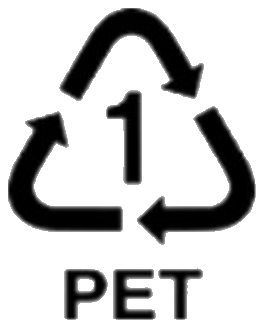
\includegraphics[width=2.4cm]{images_crop_de10/p2_cau3_pet.png}
\end{center}
\choiceTF
{\True PET thuộc loại polyester}
{\True Tơ được chế tạo từ PET thuộc loại tơ tổng hợp}
{\True Trong một mắt xích PET, phần trăm khối lượng carbon là 62,5\%}
{Phản ứng tổng hợp PET từ terephthalic acid và ethylene glycol thuộc loại phản ứng trùng hợp}
\loigiai{
a) \textbf{Đúng}. PET chứa các liên kết ester \ce{-COO-} trong mạch chính nên thuộc loại polyester.\\
b) \textbf{Đúng}. Tơ lapsan (dacron) sản xuất từ PET là tơ tổng hợp.\\
c) \textbf{Đúng}. Một mắt xích PET có công thức phân tử là \ce{C10H8O4} ($M = 192\text{ amu}$).\\
Phần trăm khối lượng carbon là:
$$\%C = \frac{10 \times 12}{192} \times 100\% = 62{,}5\%.$$
d) \textbf{Sai}. Đây là phản ứng trùng ngưng giữa dicarboxylic acid và diol (tách ra các phân tử \ce{H2O}).}
\end{ex}

\begin{ex}
Công ty The Goodyear Tire \& Rubber là một trong những công ty lốp xe lớn nhất thế giới khởi lập năm 1898. Năm 1971, lốp Goodyear trở thành bánh xe đầu tiên lăn trên Mặt Trăng\dots{} Tên công ty được đặt theo tên của nhà tiên phong Charles Goodyear, người khám phá ra phương pháp kết hợp giữa nguyên tố S (lưu huỳnh) với cao su để tạo ra một loại cao su mới.
\choiceTF
{\True Loại cao su này có tên là cao su lưu hóa}
{Cao su lưu hóa có cấu trúc mạch phân nhánh}
{\True Cao su lưu hóa làm tăng cao tính bền hơn với nhiệt và các tác nhân khác, độ đàn hồi cao, chống thấm khí, chống thấm ẩm, tăng khả năng chịu được sự ma sát, va chạm tốt hơn cao su thiên nhiên}
{Cao su lưu hóa làm tăng tính bền cơ học nhờ các cầu nối trisulfide (\ce{-S-S-S-}) giữa các phân tử polyisoprene}
\loigiai{
a) \textbf{Đúng}. Cao su tác dụng với lưu huỳnh tạo thành cao su lưu hóa.\\
b) \textbf{Sai}. Cao su lưu hóa có cấu trúc mạng không gian 3 chiều.\\
c) \textbf{Đúng}. Quá trình lưu hóa nâng cao độ đàn hồi, độ chịu nhiệt và độ bền cơ học.\\
d) \textbf{Sai}. Cầu nối giữa các mạch phân tử là cầu disulfide (\ce{-S-S-}) hoặc monosulfide (\ce{-S-}), không phải trisulfide.}
\end{ex}



\noindent
\textbf{PHẦN III (1,5 điểm -- 6 câu): Câu trắc nghiệm yêu cầu trả lời ngắn.}\\
\textit{Thí sinh trả lời từ câu 1 đến câu 6.}

\setcounter{ex}{0}

\begin{ex}
(SBT -- CTST). Có bao nhiêu loại polymer có thể tạo thành từ adipic acid, 1,2-ethylene diamine và ethylene glycol bằng phản ứng trùng ngưng?
\par\noindent\textbf{Đáp số:} \textbf{\color{red}2}
\loigiai{
Có 2 loại polymer có thể tạo thành:\\
- Adipic acid phản ứng với 1,2-ethylene diamine tạo thành polyamide.\\
- Adipic acid phản ứng với ethylene glycol tạo thành polyester.\\
(1,2-ethylene diamine và ethylene glycol không trùng ngưng với nhau).\\
\textbf{Đáp số: 2.}}
\end{ex}

\begin{ex}
Cho dãy các polymer sau: polyethylene, cellulose, nylon-6,6, amylose, nylon-6, tơ nitron, polybuta-1,3-diene, tơ visco, poly(phenol formaldehyde), poly(vinyl acetate). Có bao nhiêu polymer tổng hợp trong dãy trên?
\par\noindent\textbf{Đáp số:} \textbf{\color{red}7}
\loigiai{
Các polymer tổng hợp gồm 7 chất: polyethylene, nylon-6,6, nylon-6, tơ nitron, polybuta-1,3-diene, poly(phenol formaldehyde), poly(vinyl acetate).\\
(Cellulose và amylose là polymer thiên nhiên; tơ visco là polymer bán tổng hợp).\\
\textbf{Đáp số: 7.}}
\end{ex}

\begin{ex}
Khối lượng phân tử của một loại thủy tinh hữu cơ plexiglass là 25000 amu. Số mắt xích trong phân tử thủy tinh hữu cơ đó là bao nhiêu?
\par\noindent\textbf{Đáp số:} \textbf{\color{red}250}
\loigiai{
Thủy tinh hữu cơ plexiglass là poly(methyl methacrylate) có mắt xích là \ce{[-CH2-C(CH3)(COOCH3)-]}.\\
Khối lượng phân tử của một mắt xích là:
$$M = 5 \times 12 + 8 \times 1 + 2 \times 16 = 100\text{ amu.}$$
Số mắt xích trong phân tử polymer là:
$$n = \frac{25000}{100} = 250.$$
\textbf{Đáp số: 250.}}
\end{ex}

\begin{ex}
Khối lượng phân tử của một đoạn polyethylene (PE) là 28000 amu. Số mắt xích của đoạn polymer này là bao nhiêu?
\par\noindent\textbf{Đáp số:} \textbf{\color{red}1000}
\loigiai{
Polyethylene có dạng \ce{[-CH2-CH2-]_n} với phân tử khối mắt xích $M = 28\text{ amu}$.\\
Hệ số polymer hóa (số mắt xích) là:
$$n = \frac{28000}{28} = 1000.$$
\textbf{Đáp số: 1000.}}
\end{ex}

\begin{ex}
(SBT -- CTST). Cellulose triacetate được điều chế từ cellulose và acetic anhydride. Tính khối lượng cellulose triacetate (theo đơn vị tấn) tạo thành từ 1 tấn cellulose nếu hiệu suất của quá trình điều chế là 67\%. (Làm tròn kết quả đến chữ số thập phân thứ hai).
\par\noindent\textbf{Đáp số:} \textbf{\color{red}1,19}
\loigiai{
Phương trình phản ứng theo mắt xích:
$$\ce{[C6H7O2(OH)3]_n + 3n (CH3CO)2O -> [C6H7O2(OOC-CH3)3]_n + 3n CH3COOH}$$
Theo tỉ lệ mol: Cứ $162\text{ g}$ cellulose tạo thành $288\text{ g}$ cellulose triacetate.\\
Khối lượng cellulose triacetate theo lý thuyết từ 1 tấn cellulose:
$$m_{\text{LT}} = 1 \times \frac{288}{162} = 1{,}7778\text{ tấn.}$$
Khối lượng thực tế với hiệu suất $H = 67\%$:
$$m_{\text{TT}} = 1{,}7778 \times \frac{67}{100} \approx 1{,}1911\text{ tấn} \approx 1{,}19\text{ tấn.}$$
\textbf{Đáp số: 1,19.}}
\end{ex}

\begin{ex}
Một loại cao su Buna-S có phần trăm khối lượng carbon là 90,225\%; $m$ gam cao su này cộng tối đa với 9,6 gam bromine. Giá trị của $m$ (theo đơn vị gam) là bao nhiêu? (Làm tròn kết quả đến chữ số thập phân thứ hai).
\par\noindent\textbf{Đáp số:} \textbf{\color{red}5,32}
\loigiai{
Cao su Buna-S có dạng $(\ce{C4H6})_a \cdot (\ce{C8H8})_b$.\\
Phần trăm khối lượng carbon:
$$\%C = \frac{12(4a + 8b)}{54a + 104b} \times 100\% = 90{,}225\%$$
$$\Rightarrow 48a + 96b = 0{,}90225(54a + 104b) \Rightarrow 2{,}166b \approx 0{,}7215a \Rightarrow \frac{a}{b} \approx \frac{3}{1}.$$
Vậy cao su có dạng $(\ce{C4H6})_3 \cdot (\ce{C8H8})_1$.\\
Mỗi mắt xích \ce{C4H6} còn 1 liên kết đôi \ce{C=C} phản ứng với 1 phân tử \ce{Br2}:
$$n_{\ce{C4H6}} = n_{\ce{Br2}} = \frac{9{,}6}{160} = 0{,}06\text{ mol.}$$
Vì $a : b = 3 : 1$ nên $n_{\ce{C8H8}} = \frac{0{,}06}{3} = 0{,}02\text{ mol.}$\\
Khối lượng cao su là:
$$m = 0{,}06 \times 54 + 0{,}02 \times 104 = 3{,}24 + 2{,}08 = 5{,}32\text{ gam.}$$
\textbf{Đáp số: 5,32.}}
\end{ex}


\Closesolutionfile{ans}

\vspace{0.5cm}
\begin{center}
	\textbf{\Large\color{mainGreen}BẢNG TỔNG HỢP ĐÁP ÁN ĐỀ SỐ 10}
\end{center}

\vspace{0.2cm}
\noindent\textbf{\color{mainGreen}PHẦN I: TRẮC NGHIỆM NHIỀU PHƯƠNG ÁN LỰA CHỌN}
\begin{center}
\renewcommand{\arraystretch}{1.2}
\begin{tabular}{|c|c|c|c|c|c|c|c|c|c|c|c|c|c|c|c|c|c|}
\hline
\textbf{1} & \textbf{2} & \textbf{3} & \textbf{4} & \textbf{5} & \textbf{6} & \textbf{7} & \textbf{8} & \textbf{9} & \textbf{10} & \textbf{11} & \textbf{12} & \textbf{13} & \textbf{14} & \textbf{15} & \textbf{16} & \textbf{17} & \textbf{18} \\ \hline
\textbf{\color{red}C} & \textbf{\color{red}C} & \textbf{\color{red}D} & \textbf{\color{red}C} & \textbf{\color{red}D} & \textbf{\color{red}C} & \textbf{\color{red}A} & \textbf{\color{red}B} & \textbf{\color{red}C} & \textbf{\color{red}D} & \textbf{\color{red}B} & \textbf{\color{red}B} & \textbf{\color{red}B} & \textbf{\color{red}D} & \textbf{\color{red}C} & \textbf{\color{red}D} & \textbf{\color{red}D} & \textbf{\color{red}A} \\ \hline
\end{tabular}
\end{center}

\vspace{0.3cm}
\noindent\textbf{\color{mainGreen}PHẦN II: TRẮC NGHIỆM ĐÚNG SAI}
\begin{center}
\renewcommand{\arraystretch}{1.2}
\begin{tabular}{|c|c|c|c|c|}
\hline
\textbf{Câu} & \textbf{Lệnh hỏi a} & \textbf{Lệnh hỏi b} & \textbf{Lệnh hỏi c} & \textbf{Lệnh hỏi d} \\ \hline
\textbf{1} & \textbf{S} & \textbf{S} & \textbf{\color{red}Đ} & \textbf{\color{red}Đ} \\ \hline
\textbf{2} & \textbf{\color{red}Đ} & \textbf{S} & \textbf{\color{red}Đ} & \textbf{S} \\ \hline
\textbf{3} & \textbf{\color{red}Đ} & \textbf{\color{red}Đ} & \textbf{\color{red}Đ} & \textbf{S} \\ \hline
\textbf{4} & \textbf{\color{red}Đ} & \textbf{S} & \textbf{\color{red}Đ} & \textbf{S} \\ \hline
\end{tabular}
\end{center}

\vspace{0.3cm}
\noindent\textbf{\color{mainGreen}PHẦN III: TRẢ LỜI NGẮN}
\begin{center}
\renewcommand{\arraystretch}{1.2}
\begin{tabular}{|c|c|c|c|c|c|}
\hline
\textbf{Câu 1} & \textbf{Câu 2} & \textbf{Câu 3} & \textbf{Câu 4} & \textbf{Câu 5} & \textbf{Câu 6} \\ \hline
\textbf{\color{red}2} & \textbf{\color{red}7} & \textbf{\color{red}250} & \textbf{\color{red}1000} & \textbf{\color{red}1,19} & \textbf{\color{red}5,32} \\ \hline
\end{tabular}
\end{center}

\end{document}
